\documentclass{article}
\usepackage[utf8]{inputenc}
\usepackage{circuitikz}
\usepackage{float}
\usepackage{caption}
\usepackage{subcaption}

\begin{document}

%Lab 1 Fig 2

\begin{figure}%
    \centering
    \subfloat[\centering BNC Plug Connector]{{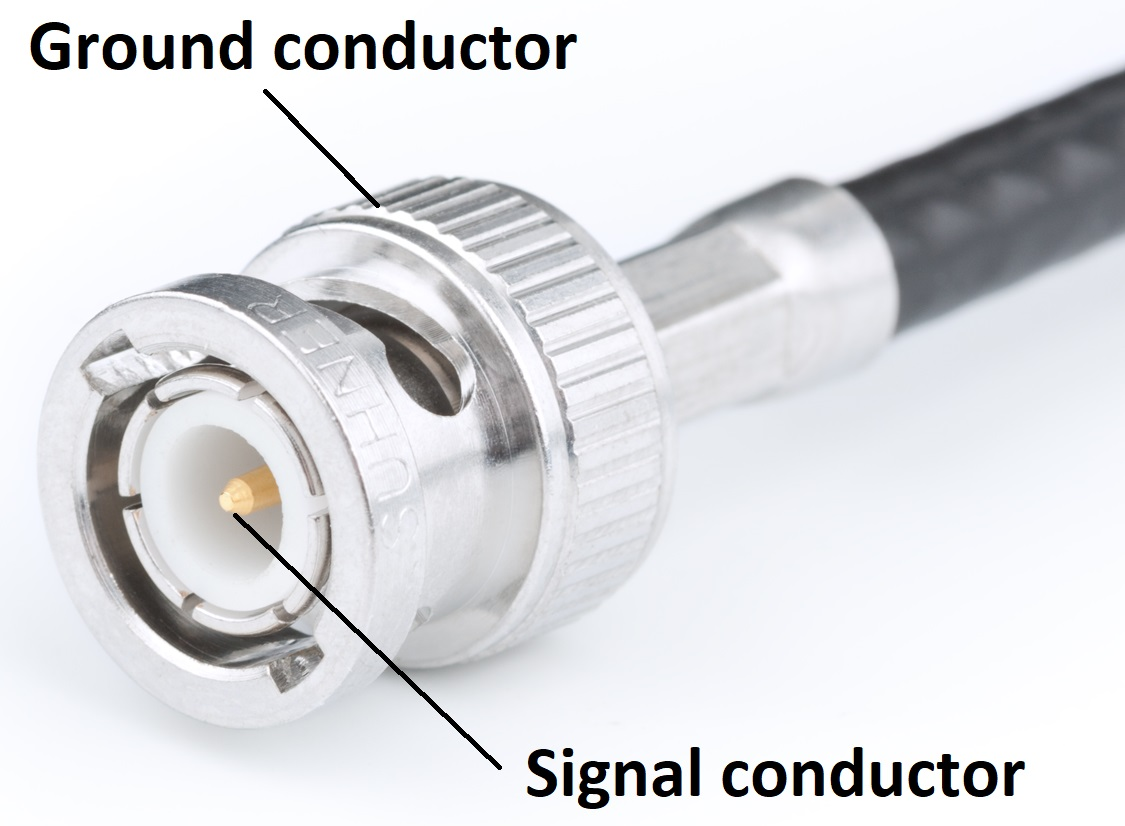
\includegraphics[width=7cm]{lab1fig/bnc-plug.jpg} }}%
    \qquad
    \subfloat[\centering Mini Grabber to BNC Socket Connector]{{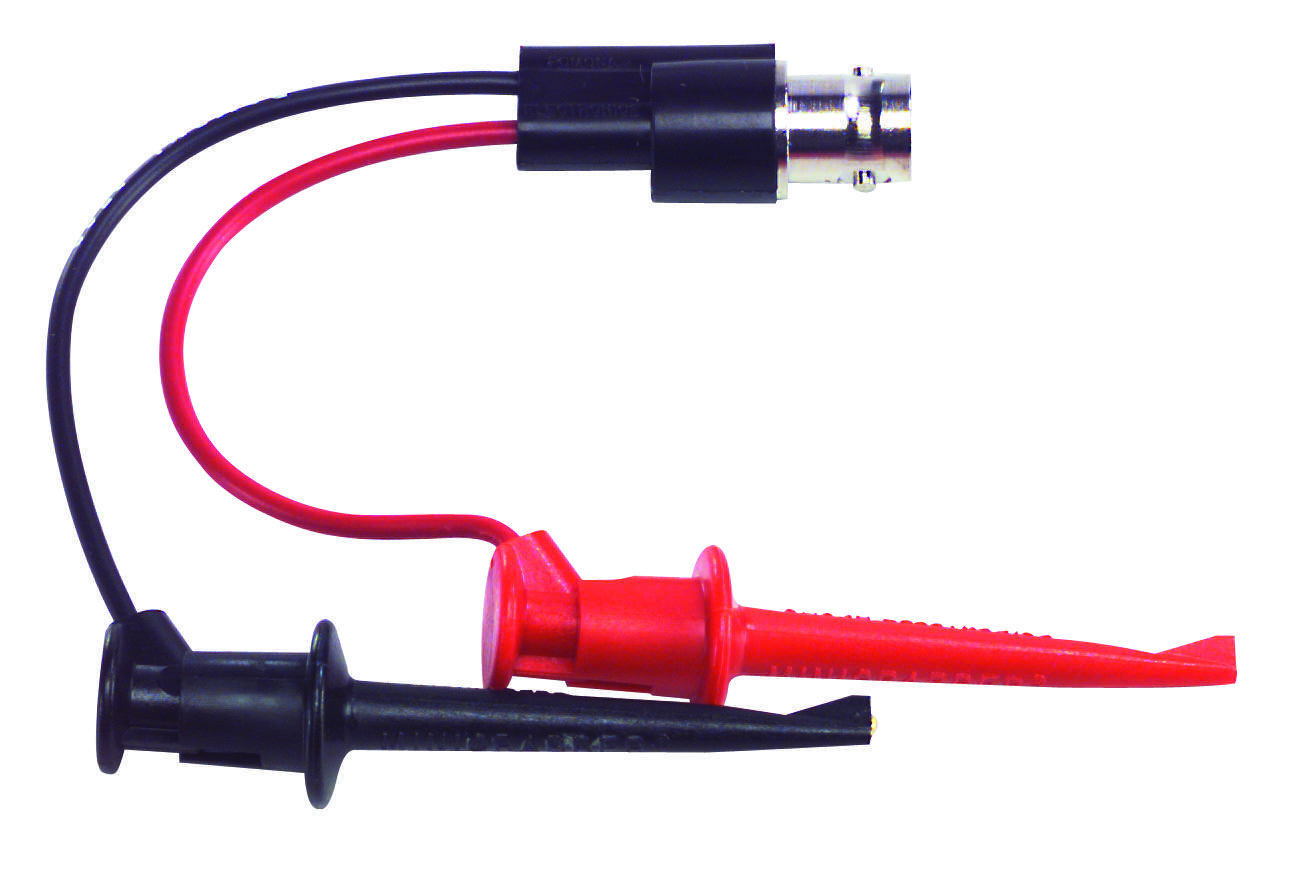
\includegraphics[width=7cm]{lab1fig/mini-grabber-to-bnc.jpg} }}%
    \caption{BNC Connector Examples}%
    \label{fig:bnc}%
\end{figure}
 
 

%Lab 2 Fig 1

\begin{figure}[h]
\centering
\begin{subfigure}[t]{0.3\textwidth}
\centering
\begin{circuitikz}[american voltages]
\draw (0,0)
    to [V, invert, *-, l=$V$] (0, 4) %-- ++(2,0)
    to [short, f=$I$] ++(2,0)
    to [R=$R_1$, -*] ++(0,-2)
    to [R=$R_2$, -*] ++(0,-2)--(0,0) node[ground]{};
    \draw (2,2) to [short, -o] (4,2) node[anchor = west]{$V_{out}$};
    \draw (2,0) to [short, -o] (4,0) node[anchor = west]{$0~V$};
\end{circuitikz}
 \caption{}
 \label{fig:a}
 \end{subfigure}
 \hspace{1.1cm}%
 \begin{subfigure}[t]{0.3\textwidth}
 \centering
\begin{circuitikz}[american voltages]
\draw (0,0)
    to [V, invert, *-, l=$V$] (0, 4) %-- ++(2,0)
    to [short, f=$I$] ++(2,0)
    to [R=$R_1$, -*] ++(0,-2)
    to [R=$R_2$, -*] ++(0,-2)--(0,0) node[ground]{};
    \draw (2,2) to [short, -o] (4.5,2) node[anchor = west]{$V_{out}$};
    \draw (2,0) to [short, -o] (4.5,0) node[anchor = west]{$0~V$};
    \draw (3.5,2) to [R=$R_3$, *-*] ++(0,-2);
\end{circuitikz}
 \caption{}
 \label{fig:b}
 \end{subfigure}
 \caption{Voltage Dividers}
 \end{figure}


\end{document}


 